%!TeX root=MemoriaTFG.tex

\chapter{Dermapixel}
\label{cap:dermapixel}

Hasta aquí los modelos se han evaluado sobre datasets públicos, casi
todos en inglés y centrados en dermatoscopia. Este capítulo da el paso
que motiva todo el trabajo: llevar esos modelos al material clínico
real con el que se quiere ayudar ---en castellano, mayoritariamente
fotografía clínica y, sobre todo, acompañado de texto---.

El origen es el blog \emph{Dermapixel}, que la Dra.~R.~Taberner
mantiene desde 2010 y que reúne más de $700$ casos comentados: cada
uno con su imagen clínica y dermatoscópica, una historia breve, el
diagnóstico y el razonamiento diferencial. Ese archivo tiene algo poco
habitual: no son solo imágenes etiquetadas, sino casos con texto
clínico rico en castellano. Y precisamente el papel de ese texto como
contexto para el diagnóstico ---la segunda vía que este trabajo
defiende como poco explorada (sección~\ref{sec:objetivos})--- es lo
que hace a Dermapixel especialmente valioso: ya tiene lo que casi
ningún dataset público ofrece.

De ahí la decisión de continuar con Dermapixel. A partir de ese
archivo se construyó DermapixelAI~1.0 (sección~\ref{sec:dermapixel})
---un dataset clínico en castellano con texto narrativo por caso--- y
se liberó para la comunidad. Este capítulo lo pone a prueba: primero
evalúa si los modelos fundacionales transfieren a este material (de
forma congelada y en zero-shot), y después presenta la
contribución propia, \textbf{Dermapixel R0}, una adaptación ligera de
PanDerm al castellano ---con una head supervisada y una rama
contrastiva imagen-texto--- cerrando con una síntesis comparativa de
todos los métodos.

\section{Evaluación de los modelos fundacionales sobre DermapixelAI}
\label{sec:dermapixel-results}

El capítulo empieza por la pregunta más básica: ¿transfieren los
modelos fundacionales a este material clínico en castellano? Esta
sección los evalúa sobre DermapixelAI~1.0 en los tres niveles de la
ontología (L1, L2 y L3): primero con sus representaciones congeladas
---usando lo que ya aprendieron, sin reentrenarlos--- y luego con una
adaptación supervisada moderada. Aparece ya un hallazgo que se repetirá
a lo largo del capítulo: no hay un método óptimo único; la mejor opción
depende del nivel de detalle diagnóstico.

Una propiedad importante de DermapixelAI~1.0 es que es completamente
independiente del preentrenamiento de PanDerm y DermLIP. A diferencia
de Dermnet (sección~\ref{sec:auditoria-resultados}), la auditoría por
hash MD5 sobre $507\,657$ imágenes catalogadas (Derm1M más los once
datasets externos del capítulo anterior) no encuentra ninguna
coincidencia ($0$ sobre las $1\,062$ imágenes evaluables). Esta
evaluación está, por tanto, libre de fuga de información (documento de
entrega del dataset en el repositorio reproducible, \ref{cap:repo},
sección~\ref{sec:repo-datasheet}).

\subsection{Transferencia congelada: linear probe y validación cruzada}

\paragraph{Linear probe sobre el split fijo.}
Se aplica el protocolo de linear probe (sección~\ref{sec:lp})
---congelar el modelo y entrenar encima solo un clasificador lineal
sencillo--- sobre las $1\,062$ imágenes evaluables (con etiqueta de
ontología y modalidad clínica o dermatoscópica; train $N = 874$,
validación $N = 152$, test $N = 36$), usando PanDerm Base ($768$-D) y
Large ($1\,024$-D) como extractores congelados. La evaluación L2 usa las $38$ subcategorías
efectivas tras consolidar las dos variantes ortográficas de
\emph{Trastornos de la queratinización} (repositorio reproducible,
\ref{cap:repo}, sección~\ref{sec:repo-ablaciones}).

\begin{table}[htbp]
\centering
\footnotesize
\setlength{\tabcolsep}{4pt}
\renewcommand{\arraystretch}{0.95}
\caption{Linear probe con PanDerm Base y Large sobre
DermapixelAI~1.0 en los tres niveles de la ontología jerárquica
($N_{\mathrm{train}} = 874$, $N_{\mathrm{test}} = 36$ en L1/L2 y
$N_{\mathrm{test}} = 28$ en L3 tras filtrar clases ausentes en
train). Entre corchetes, IC95\% por \emph{bootstrap} estratificado
($1\,000$ remuestreos). Mejor valor por columna y nivel en
negrita.}
\label{tab:dermapixel-lp}
\adjustbox{max width=\textwidth}{%
\begin{tabular}{llrrrrr}
\hline
Nivel & Modelo & Acc & BAcc & AUROC & W-F1 & Kappa \\
\hline
L1 (4 clases)   & Base  & $0{,}639$ [$0{,}472$--$0{,}778$]
                        & $0{,}570$ [$0{,}371$--$0{,}751$]
                        & $0{,}697$ [$0{,}527$--$0{,}841$]
                        & $0{,}624$ [$0{,}457$--$0{,}760$]
                        & $0{,}296$ \\
L1 (4 clases)   & Large & $\mathbf{0{,}750}$ [$0{,}639$--$0{,}861$]
                        & $\mathbf{0{,}735}$ [$0{,}637$--$0{,}835$]
                        & $\mathbf{0{,}796}$ [$0{,}656$--$0{,}930$]
                        & $\mathbf{0{,}722}$ [$0{,}596$--$0{,}845$]
                        & $\mathbf{0{,}520}$ \\
L2 (38 clases)  & Base  & $0{,}222$ [$0{,}139$--$0{,}333$]
                        & $0{,}221$ [$0{,}147$--$0{,}294$]
                        & $0{,}707$ [$0{,}666$--$0{,}747$]
                        & $0{,}212$ [$0{,}092$--$0{,}302$]
                        & $0{,}170$ \\
L2 (38 clases)  & Large & $\mathbf{0{,}250}$ [$0{,}167$--$0{,}333$]
                        & $\mathbf{0{,}265}$ [$0{,}206$--$0{,}338$]
                        & $\mathbf{0{,}793}$ [$0{,}749$--$0{,}837$]
                        & $\mathbf{0{,}223}$ [$0{,}139$--$0{,}291$]
                        & $\mathbf{0{,}199}$ \\
L3 (224 clases) & Base  & $0{,}143$ [$0{,}107$--$0{,}179$]
                        & $0{,}132$ [$0{,}105$--$0{,}158$]
                        & $0{,}735$ [$0{,}693$--$0{,}779$]
                        & $0{,}107$ [$0{,}064$--$0{,}141$]
                        & $0{,}112$ \\
L3 (224 clases) & Large & $\mathbf{0{,}179}$ [$0{,}143$--$0{,}214$]
                        & $\mathbf{0{,}184}$ [$0{,}158$--$0{,}211$]
                        & $\mathbf{0{,}813}$ [$0{,}769$--$0{,}856$]
                        & $\mathbf{0{,}143}$ [$0{,}100$--$0{,}184$]
                        & $\mathbf{0{,}154}$ \\
\hline
\end{tabular}}
\end{table}

De aquí salen dos lecturas claras. La primera: PanDerm Large vuelve a
ser mejor que Base en las cinco métricas y los tres niveles, igual que
sobre los datasets externos. La segunda: cuanto más fino es el
diagnóstico, más cuesta ---la BAcc de Large baja de $0{,}735$ (L1,
cuatro grandes familias) a $0{,}265$ (L2) y $0{,}184$ (L3, $224$
diagnósticos)---, aunque incluso en L3 el modelo acierta casi $41$
veces más que el azar ($2{,}9\times$ en L1, $10{,}2\times$ en L2,
$40{,}9\times$ en L3). El rendimiento en L1 (BAcc $0{,}735$, IC95\%
[$0{,}637$--$0{,}835$]) cae dentro del rango de los diez datasets
externos (tabla~\ref{tab:lp-panderm}): DermapixelAI~1.0 es, por tanto,
un benchmark exigente en castellano y sin las marcas
estandarizadas de la dermatoscopia.


\paragraph{Validación cruzada agrupada por caso.}
Como el test fijo ($N = 36$) es una única partición, se estima el
rendimiento esperado con validación cruzada de cinco \emph{folds}: se
reparten las $1\,062$ imágenes en cinco grupos ---respetando las
proporciones de cada familia L1 y manteniendo juntas todas las imágenes
de un mismo caso---, de modo que ninguna imagen del mismo paciente caiga
a la vez en train y test. La tabla~\ref{tab:dermapixel-cv} reporta media
y desviación sobre los cinco \emph{folds}.

\begin{table}[htbp]
\centering
\footnotesize
\setlength{\tabcolsep}{4pt}
\renewcommand{\arraystretch}{0.95}
\caption{Validación cruzada agrupada por caso (cinco \emph{folds},
estratificado por L1 sobre \texttt{case\_id}) con PanDerm Large
sobre DermapixelAI~1.0. Cifras: media $\pm$ desviación estándar
sobre los cinco \emph{folds}. La cardinalidad L3 reportada aquí
(250 clases) corresponde a las clases efectivas en el dataset
completo; las restantes tablas del split fijo
(tabla~\ref{tab:dermapixel-lp}, tabla~\ref{tab:dermapixel-ensemble}
y las del repositorio reproducible, \ref{sec:repo-ablaciones}) usan 224 clases L3, las
únicas representadas en el split \texttt{train}.}
\label{tab:dermapixel-cv}
\begin{tabular}{lrrrrrr}
\hline
Nivel           & Acc@1                 & Acc@3                 & BAcc                  & AUROC                 & W-F1                  & Kappa \\
\hline
L1 (4 cls)      & $0{,}574 \pm 0{,}029$ & $0{,}994 \pm 0{,}004$ & $0{,}440 \pm 0{,}058$ & $0{,}753 \pm 0{,}054$ & $0{,}569 \pm 0{,}025$ & $0{,}314 \pm 0{,}035$ \\
L2 (38 cls)     & $0{,}227 \pm 0{,}015$ & $0{,}418 \pm 0{,}037$ & $0{,}168 \pm 0{,}020$ & $0{,}749 \pm 0{,}019$ & $0{,}221 \pm 0{,}022$ & $0{,}186 \pm 0{,}015$ \\
L3 (250 cls)    & $0{,}124 \pm 0{,}007$ & $0{,}232 \pm 0{,}028$ & $0{,}108 \pm 0{,}014$ & $0{,}800 \pm 0{,}018$ & $0{,}124 \pm 0{,}005$ & $0{,}110 \pm 0{,}005$ \\
\hline
\end{tabular}
\end{table}

Con un test de solo $36$ imágenes conviene no fiarse de una única
partición. Por eso la validación cruzada agrupada por caso ---que
reparte los casos en cinco grupos sin que dos imágenes del mismo
paciente caigan a la vez en train y test--- es la
estimación más honesta del rendimiento esperable. Comparado con ella,
el test fijo resulta optimista en BAcc ($+29{,}5$\,pp en L1,
$+9{,}7$\,pp en L2, $+7{,}6$\,pp en L3) porque le tocó un reparto
favorable; la AUROC, en cambio, apenas cambia con la partición (menos
de $5$\,pp). Las cifras del test fijo (tabla~\ref{tab:dermapixel-lp})
se conservan como punto operativo y como base de comparación con el
experimento zero-shot (sección~\ref{sec:dermapixel-zs}), que usa
el mismo test.


\subsection{Validación del procedimiento de etiquetado}

Parte de las etiquetas de nivel L1 viene de la ontología y no de una
revisión imagen a imagen, así que conviene comprobar que eso no falsea
los resultados. Se compara el linear probe sobre el subconjunto
revisado por la Dra.~Taberner (\texttt{rosa\_verified}) frente al
dataset completo: las diferencias son pequeñas y sin un sentido claro,
compatibles con el azar de la muestra. El etiquetado por ontología no
degrada, por tanto, el rendimiento (detalle en el repositorio
reproducible, \ref{cap:repo}, sección~\ref{sec:repo-ablaciones}).

Sobre esos mismos embeddings se probaron además varias técnicas de
apoyo, todas sencillas: usar como clasificador final un k-NN o un
pequeño MLP en vez del lineal; cambiar la función de pérdida; dar más
peso a las clases poco frecuentes (class weight); y aplicar TTA
(test-time augmentation), que promedia las predicciones sobre varias
versiones aumentadas de cada imagen para estabilizar el resultado.
Ninguna cambia las conclusiones, y todas se documentan en el mismo
repositorio.


\subsection{Estrategias de adaptación más allá del linear probe}
\label{sec:dermapixel-ensemble}

Más allá de la representación congelada, dos estrategias buscan mejorar
el rendimiento sobre DermapixelAI~1.0: combinar encoders
complementarios y ajustar finamente el encoder.

\paragraph{Combinación de encoders.}
Para ver si distintos encoders se complementan, se entrena un
clasificador lineal sobre cada uno (PanDerm Base, Large y DermLIP v2;
protocolo de sección~\ref{sec:lp}) y se comparan con cinco formas de
combinarlos: promediar sus predicciones (las tres, o solo
Large$+$DermLIP), quedarse con la clase de mayor puntuación entre los
tres, o un \emph{apilado} ---un segundo clasificador que aprende a
fusionarlas---. La
tabla~\ref{tab:dermapixel-ensemble} reporta los tres niveles en el
mismo test fijo.

\begin{table}[htbp]
\centering
\footnotesize
\setlength{\tabcolsep}{4pt}
\renewcommand{\arraystretch}{0.95}
\caption{Combinación de encoders sobre DermapixelAI~1.0. LP
individual sobre PanDerm Base, PanDerm Large y DermLIP v2; tres
estrategias de combinación: promedio Large$+$DermLIP, máximo por
clase entre los tres, y apilado con meta-head. Mejor valor por
columna y nivel en negrita.}
\label{tab:dermapixel-ensemble}
\begin{tabular}{llrrrr}
\hline
Nivel & Estrategia                         & Acc@1              & Acc@3              & BAcc               & AUROC \\
\hline
L1 (4 cls)   & LP PanDerm Base             & $0{,}639$          & ---                & $0{,}570$          & $0{,}697$ \\
L1 (4 cls)   & LP PanDerm Large            & $\mathbf{0{,}750}$ & $\mathbf{1{,}000}$ & $\mathbf{0{,}735}$ & $0{,}796$ \\
L1 (4 cls)   & LP DermLIP v2               & $0{,}694$          & $\mathbf{1{,}000}$ & $0{,}680$          & $0{,}789$ \\
L1 (4 cls)   & Avg L$+$D                   & $\mathbf{0{,}750}$ & $\mathbf{1{,}000}$ & $0{,}702$          & $\mathbf{0{,}817}$ \\
L1 (4 cls)   & Avg 3                       & $0{,}722$          & $\mathbf{1{,}000}$ & $0{,}694$          & $0{,}811$ \\
L1 (4 cls)   & Máx 3                       & $0{,}694$          & $\mathbf{1{,}000}$ & $0{,}652$          & $0{,}805$ \\
L1 (4 cls)   & Stack 3                     & $0{,}694$          & $\mathbf{1{,}000}$ & $0{,}703$          & $0{,}790$ \\
\hline
L2 (38 cls)  & LP PanDerm Base             & $0{,}222$          & ---                & $0{,}221$          & $0{,}707$ \\
L2 (38 cls)  & LP PanDerm Large            & $0{,}250$          & $0{,}500$          & $0{,}265$          & $0{,}793$ \\
L2 (38 cls)  & LP DermLIP v2               & $\mathbf{0{,}333}$ & $0{,}528$          & $\mathbf{0{,}279}$ & $\mathbf{0{,}860}$ \\
L2 (38 cls)  & Avg L$+$D                   & $0{,}278$          & $\mathbf{0{,}556}$ & $\mathbf{0{,}279}$ & $0{,}832$ \\
L2 (38 cls)  & Avg 3                       & $0{,}278$          & $0{,}528$          & $0{,}268$          & $0{,}821$ \\
L2 (38 cls)  & Máx 3                       & $0{,}222$          & $0{,}528$          & $0{,}235$          & $0{,}797$ \\
L2 (38 cls)  & Stack 3                     & $0{,}250$          & $0{,}528$          & $0{,}258$          & $0{,}804$ \\
\hline
L3 (224 cls) & LP PanDerm Base             & $0{,}143$          & ---                & $0{,}132$          & $0{,}735$ \\
L3 (224 cls) & LP PanDerm Large            & $\mathbf{0{,}179}$ & $\mathbf{0{,}286}$ & $\mathbf{0{,}184}$ & $\mathbf{0{,}813}$ \\
L3 (224 cls) & LP DermLIP v2               & $0{,}107$          & $0{,}214$          & $0{,}079$          & $0{,}809$ \\
L3 (224 cls) & Avg L$+$D                   & $\mathbf{0{,}179}$ & $0{,}250$          & $\mathbf{0{,}184}$ & $0{,}802$ \\
L3 (224 cls) & Avg 3                       & $0{,}143$          & $0{,}250$          & $0{,}152$          & $0{,}795$ \\
L3 (224 cls) & Máx 3                       & $0{,}143$          & $0{,}250$          & $0{,}132$          & $0{,}780$ \\
L3 (224 cls) & Stack 3                     & $0{,}143$          & $0{,}250$          & $0{,}158$          & $0{,}791$ \\
\hline
\end{tabular}
\end{table}

Ningún encoder gana en los tres niveles a la vez. En L1 gana la
combinación avg Large$+$DermLIP en AUROC ($0{,}796 \to 0{,}817$); en L2,
DermLIP v2 él solo en todas las métricas ($+6{,}7$\,pp AUROC sobre
PanDerm Large, $0{,}793 \to 0{,}860$), sin que ninguna combinación lo
mejore (coherente con el experimento zero-shot,
sección~\ref{sec:dermapixel-zs}); en L3 gana PanDerm Large solo, donde
la long tail deja poca señal que combinar. Lo que se aprende: combinar
encoders ayuda a veces, pero no hay un montaje único que sea el mejor
en todo.


\paragraph{Fine-tuning parcial del encoder.}
\label{sec:dermapixel-ft}
\label{sec:dermapixel-ft-l1}
Este protocolo repite sobre DermapixelAI~1.0 el fine-tuning supervisado
(FT) de la sección~\ref{sec:ft-results}: en vez de congelar PanDerm
Large entero, se descongelan sus dos últimas capas ($25{,}2$\,M
parámetros, el $8{,}3\%$ del modelo) y se entrena un clasificador
encima, dando más peso a la clase minoritaria (\emph{Genodermatosis})
para compensar que tiene muy pocos ejemplos (receta en el repositorio
reproducible, \ref{cap:repo}, sección~\ref{sec:repo-reproducibilidad}).

Sobre el nivel L1, el fine-tuning parcial alcanza BAcc $0{,}622$
(IC95\% [$0{,}510$--$0{,}735$]) y AUROC $0{,}715$, lo que mejora en
$+18{,}2$\,pp la cifra de validación cruzada agrupada por caso del
linear probe congelado (BAcc $0{,}440 \pm 0{,}058$,
tabla~\ref{tab:dermapixel-cv}), con intervalos no solapados: el
fine-tuning aporta valor real más allá del ruido de partición. No
obstante, no supera a la combinación lineal de encoders
congelados \texttt{avg\_large\_dermlip}
(sección~\ref{sec:dermapixel-ensemble}; BAcc $0{,}702$, AUROC
$0{,}817$). La replicación sobre L2 y L3 mantiene el mismo
protocolo, variando únicamente la head supervisada. La
tabla~\ref{tab:dermapixel-ft-multilevel} compara las métricas
sobre los tres niveles.

\begin{table}[htbp]
\centering
\footnotesize
\setlength{\tabcolsep}{4pt}
\renewcommand{\arraystretch}{0.95}
\caption{Fine-tuning parcial del encoder (PanDerm Large, dos
últimas capas descongeladas) sobre los tres niveles ontológicos de
DermapixelAI~1.0. Test fijo $N_{\mathrm{test}} = 36$ en L1/L2 y
$N_{\mathrm{test}} = 28$ en L3. La head L2 de este protocolo
dimensiona $1\,024 \to 37$: son las $37$ clases L2 efectivas en el
\emph{train} del fine-tuning, de las $38$ del dataset tras fusionar
las dos variantes ortográficas de ``queratinización'' ($39$ en
bruto); las $38$ clases son la cardinalidad nominal del nivel L2.
Entre corchetes, IC95\% por \emph{bootstrap}
estratificado ($1\,000$ remuestreos). Mejor valor por columna en
negrita.}
\label{tab:dermapixel-ft-multilevel}
\begin{tabular}{lrrrr}
\hline
Nivel        & Acc@1                            & Acc@3                            & BAcc                             & AUROC \\
\hline
L1 (4 cls)   & $\mathbf{0{,}583}$ [$0{,}444$--$0{,}722$] & $\mathbf{0{,}972}$ [$0{,}917$--$1{,}000$] & $\mathbf{0{,}622}$ [$0{,}510$--$0{,}735$] & $0{,}715$ [$0{,}603$--$0{,}830$] \\
L2 (37 cls)  & $0{,}250$ [$0{,}167$--$0{,}333$] & $0{,}500$ [$0{,}389$--$0{,}611$] & $0{,}324$ [$0{,}265$--$0{,}397$] & $\mathbf{0{,}852}$ [$0{,}814$--$0{,}888$] \\
L3 (224 cls) & $0{,}179$ [$0{,}143$--$0{,}214$] & $0{,}286$ [$0{,}214$--$0{,}357$] & $0{,}184$ [$0{,}158$--$0{,}211$] & $0{,}804$ [$0{,}773$--$0{,}835$] \\
\hline
\end{tabular}
\end{table}

El fine-tuning parcial mejora al linear probe en L1 y L2, pero no es la
adaptación más eficiente: la versión con LoRA de Dermapixel R0
(sección~\ref{sec:dermapixel-spanderm-v0}) rinde mejor entrenando
muchos menos parámetros. En conjunto, ni combinar encoders ni el
fine-tuning dan una opción mejor para todo: \textbf{el rendimiento
depende a la vez del nivel ontológico, de cómo se adapta el modelo y de
qué métrica se mire}, así que buscar un único encoder ``ganador'' es
simplificar de más (lectura de diseño en
sección~\ref{sec:disc-especializacion}).

\subsection{Limitaciones del fine-tuning en la long tail}

Sobre el nivel L3, el fine-tuning denso parcial no supera al linear probe congelado (BAcc $0{,}184$ en ambos): la long tail severa del
nivel ($193$ de las $250$ clases L3 efectivas, el $77\%$, con $\leq 5$
imágenes) anula el beneficio
del fine-tuning, lo que reserva L3 al ranking por prototipos coseno de
Dermapixel R0 (repositorio reproducible, \ref{cap:repo}, sección~\ref{sec:repo-ablaciones}) o a la
ampliación del dataset vía banco hospitalario del HUSLL.

Tres caveats acotan estas cifras: el test reducido ($N = 36$
en L1/L2, $N = 28$ en L3) ensancha los IC95\%; la ausencia de
\emph{Genodermatosis} en el test de L1 ($0 / 36$) reduce ese nivel a
una clasificación efectiva de tres clases; y la long tail de L3
limita el rendimiento alcanzable bajo cualquier ajuste denso sobre el
dataset actual.

En conjunto, esta primera prueba sobre material clínico en castellano
deja tres ideas claras. La primera: PanDerm Large transfiere bien al
grano grueso ---las cuatro grandes familias de L1--- y el problema se
endurece de forma ordenada a medida que el diagnóstico se afina (L2 y,
sobre todo, L3), aunque siempre muy por encima del azar. La segunda:
ninguna de las recetas probadas ---linear probe congelado, combinación
de encoders o fine-tuning parcial--- gana en todos los niveles a la vez;
cuál conviene depende del nivel de detalle y de la métrica que se
priorice, de modo que hablar de un único encoder ``ganador'' simplifica
de más. Y la tercera: en el nivel más fino el cuello de botella deja de
ser el modelo y pasa a ser el dato ---la long tail de diagnósticos
raros---, lo que explica por qué la adaptación eficiente de Dermapixel R0
(sección~\ref{sec:dermapixel-spanderm-v0}) y la futura ampliación con el
banco hospitalario (sección~\ref{sec:dermapixel-futuro}) son los caminos
naturales para crecer.

\section{Validación zero-shot multimodal sobre DermapixelAI 1.0}
\label{sec:dermapixel-zs}

Esta sección pregunta lo contrario que la anterior: ¿hasta dónde llega
un modelo fundacional sobre el material en castellano \emph{sin
entrenar nada}, solo describiendo cada diagnóstico con palabras? La
distancia entre este régimen zero-shot y el supervisado depende
mucho del nivel de detalle: es grande en L1 y L3, pero casi desaparece
en L2 ---el resultado más llamativo de la sección---, donde DermLIP v2
en zero-shot alcanza una AUROC ($0{,}794$) indistinguible de la
del linear probe supervisado de PanDerm Large ($0{,}793$).

El experimento usa el mismo test que la
sección~\ref{sec:dermapixel-results} ($N_{\mathrm{test}} = 36$ en
L1/L2, $28$ en L3), sin entrenar ningún clasificador y con no
solapamiento garantizado ($0 / 507\,657$ coincidencias MD5). Se
comparan tres modelos contrastivos ---DermLIP v2 (Derm1M),
SigLIP-SO400M (WebLI) y BiomedCLIP (PubMed-15M)--- eligiendo para cada
imagen la clase de mayor similitud coseno con un ensemble de
tres plantillas de texto por nivel, y se contrasta el prompt en
castellano frente al inglés; L3 se evalúa solo en castellano por falta
de una traducción inglesa validada de sus $224$ clases
(tabla~\ref{tab:dermapixel-zs}).

\begin{table}[htbp]
\centering
\footnotesize
\setlength{\tabcolsep}{4pt}
\renewcommand{\arraystretch}{0.95}
\caption{Clasificación \emph{zero-shot} multimodal sobre el
conjunto de test de DermapixelAI~1.0 ($N_{\mathrm{test}} = 36$ en
L1/L2, $N_{\mathrm{test}} = 28$ en L3). Entre corchetes, IC95\%
por \emph{bootstrap} estratificado ($1\,000$ remuestreos) para
las dos métricas primarias (Acc@1 y AUROC). Las métricas BAcc y
Acc@3 se reportan como valor puntual por concisión; los IC95\%
correspondientes están disponibles en el material reproducible.
L3 se evalúa únicamente en castellano. Mejor valor por columna,
nivel e idioma en negrita.}
\label{tab:dermapixel-zs}
\begin{tabular}{lllrrrr}
\hline
Nivel & Modelo & Lang & Acc@1 & Acc@3 & BAcc & AUROC \\
\hline
L1 (4 cls)   & BiomedCLIP    & es & $\mathbf{0{,}389}$ [$0{,}250$--$0{,}528$]
                                  & $\mathbf{0{,}944}$
                                  & $0{,}375$
                                  & $0{,}679$ [$0{,}562$--$0{,}781$] \\
L1 (4 cls)   & BiomedCLIP    & en & $0{,}389$ [$0{,}250$--$0{,}528$]
                                  & $\mathbf{0{,}972}$
                                  & $0{,}324$
                                  & $0{,}639$ [$0{,}524$--$0{,}738$] \\
L1 (4 cls)   & SigLIP-SO400M & es & $0{,}222$ [$0{,}111$--$0{,}361$]
                                  & $0{,}917$
                                  & $0{,}178$
                                  & $0{,}650$ [$0{,}571$--$0{,}735$] \\
L1 (4 cls)   & SigLIP-SO400M & en & $0{,}333$ [$0{,}194$--$0{,}472$]
                                  & $0{,}889$
                                  & $0{,}292$
                                  & $0{,}663$ [$0{,}595$--$0{,}719$] \\
L1 (4 cls)   & DermLIP v2    & es & $0{,}361$ [$0{,}222$--$0{,}500$]
                                  & $0{,}861$
                                  & $0{,}379$
                                  & $0{,}699$ [$0{,}600$--$0{,}794$] \\
L1 (4 cls)   & DermLIP v2    & en & $\mathbf{0{,}500}$ [$0{,}333$--$0{,}667$]
                                  & $0{,}917$
                                  & $\mathbf{0{,}441}$
                                  & $\mathbf{0{,}709}$ [$0{,}565$--$0{,}841$] \\
\hline
L2 (38 cls)  & BiomedCLIP    & es & $0{,}111$ [$0{,}111$--$0{,}111$]
                                  & $0{,}278$
                                  & $0{,}118$
                                  & $0{,}647$ [$0{,}604$--$0{,}688$] \\
L2 (38 cls)  & BiomedCLIP    & en & $0{,}083$ [$0{,}056$--$0{,}111$]
                                  & $0{,}250$
                                  & $0{,}088$
                                  & $0{,}655$ [$0{,}601$--$0{,}713$] \\
L2 (38 cls)  & SigLIP-SO400M & es & $0{,}139$ [$0{,}139$--$0{,}139$]
                                  & $0{,}250$
                                  & $0{,}235$
                                  & $0{,}636$ [$0{,}589$--$0{,}680$] \\
L2 (38 cls)  & SigLIP-SO400M & en & $0{,}194$ [$0{,}111$--$0{,}278$]
                                  & $0{,}278$
                                  & $0{,}221$
                                  & $0{,}697$ [$0{,}640$--$0{,}747$] \\
L2 (38 cls)  & DermLIP v2    & es & $\mathbf{0{,}222}$ [$0{,}167$--$0{,}278$]
                                  & $0{,}333$
                                  & $0{,}265$
                                  & $0{,}762$ [$0{,}721$--$0{,}805$] \\
L2 (38 cls)  & DermLIP v2    & en & $\mathbf{0{,}250}$ [$0{,}194$--$0{,}306$]
                                  & $\mathbf{0{,}417}$
                                  & $\mathbf{0{,}294}$
                                  & $\mathbf{0{,}794}$ [$0{,}747$--$0{,}837$] \\
\hline
L3 (224 cls) & BiomedCLIP    & es & $0{,}107$ [$0{,}036$--$0{,}179$]
                                  & $0{,}214$
                                  & $0{,}079$
                                  & $0{,}703$ [$0{,}673$--$0{,}732$] \\
L3 (224 cls) & SigLIP-SO400M & es & $0{,}071$ [$0{,}000$--$0{,}143$]
                                  & $0{,}214$
                                  & $0{,}053$
                                  & $0{,}696$ [$0{,}667$--$0{,}723$] \\
L3 (224 cls) & DermLIP v2    & es & $\mathbf{0{,}107}$ [$0{,}071$--$0{,}143$]
                                  & $\mathbf{0{,}214}$
                                  & $\mathbf{0{,}079}$
                                  & $\mathbf{0{,}740}$ [$0{,}719$--$0{,}763$] \\
\hline
\end{tabular}
\end{table}

La evaluación zero-shot sobre DermapixelAI~1.0 deja tres
hallazgos principales.

\textit{Primero, el mejor modelo en este material es DermLIP v2:} gana o
empata en las cinco métricas y los tres niveles ---la única excepción es
Acc@3 en L1, donde lidera BiomedCLIP---. No sorprende, porque es el único
de los tres que se preentrenó específicamente con imágenes de
dermatología (Derm1M~\cite{derm1m}). Es, de hecho, el modelo que el
prototipo DermApIxel emplea para su módulo de clasificación zero-shot de
clase abierta (sección~\ref{sec:repo-prototipo}).

\textit{Segundo, escribir el \emph{prompt} en castellano en vez de en
inglés penaliza a los modelos entrenados en inglés:} la Acc@1 en L1 cae
entre $11$ y $14$ puntos (DermLIP v2 pierde $13{,}9$\,pp, de $0{,}500$ a
$0{,}361$; SigLIP-SO400M, $11{,}1$\,pp), mientras que BiomedCLIP rinde
igual en ambos idiomas. Encaja con que esos modelos vieron sobre todo
texto en inglés durante el preentrenamiento ---aunque el experimento no
permite atribuir la caída únicamente a ese factor--- y es justo lo que
justifica dotar a Dermapixel R0 de una rama de texto en castellano: si el
idioma no penalizara, esa rama no tendría sentido.

\textit{Tercero, en una franja concreta el modelo sin entrenar alcanza al
modelo entrenado.} Comparar el régimen zero-shot con el linear probe
supervisado (tabla~\ref{tab:dermapixel-lp}) mide cuánto se gana por
entrenar: $+29{,}4$\,pp de BAcc en L1 y $+10{,}5$\,pp en L3 a favor del
modelo entrenado. En L2, sin embargo, esa ventaja casi desaparece, y ahí
está el resultado más llamativo de la sección: DermLIP v2 sin entrenar
nada, describiendo cada diagnóstico con palabras en inglés (AUROC
$0{,}794$), iguala al mejor modelo entrenado (PanDerm Large, $0{,}793$)
dentro de los intervalos de confianza. La lectura es que, en el grano
intermedio de las subcategorías, buena parte del conocimiento necesario
para distinguirlas ya está dentro del modelo preentrenado y se puede
recuperar con texto, sin entrenar; el grano grueso (L1) y la cola de
diagnósticos raros (L3) sí siguen necesitando un clasificador entrenado.
La tabla que resume estas brechas ---penalización por idioma y distancia
al linear probe--- está en el repositorio reproducible (\ref{cap:repo},
sección~\ref{sec:repo-ablaciones}).

Las cautelas sobre el tamaño del test ($N = 36$ en L1/L2, $N = 28$ en L3)
y la ausencia de solapamiento con Derm1M
(sección~\ref{sec:dermapixel-results}) valen también aquí. Hay además dos
propias del régimen zero-shot. Una: para describir cada clase se usaron
solo tres plantillas de texto por nivel, una versión deliberadamente
mínima ---la literatura suele emplear entre diez y ochenta plantillas
generadas con ayuda de LLMs---, así que estas cifras son un suelo, no un
techo. Y otra: L3 se evaluó solo en castellano, porque no se dispone de
una traducción inglesa validada de sus $224$ clases, lo que impide medir
la penalización por idioma sobre la long tail.

\section{Dermapixel R0: adaptación supervisada con LoRA (nivel L2)}
\label{sec:dermapixel-spanderm-v0}

Llegamos al primer modelo propio.
\textbf{Dermapixel R0} es la primera adaptación de PanDerm al
castellano, y conviene decir desde el principio qué cabe esperar de
ella ---y qué no---. Sabemos que las cifras serán modestas, por dos
razones honestas: el dataset es pequeño (alrededor de mil imágenes, con
una larga cola de diagnósticos de muy pocos ejemplos) y PanDerm se
preentrenó sobre material mayoritariamente en inglés, así que llevarlo
hacia el castellano es empezar cuesta arriba. La gracia, por tanto, no
es batir ningún récord: es \emph{empezar}. R0 ---la ``versión cero''---
busca demostrar que se puede especializar un modelo fundacional al
castellano con recursos muy modestos y dejar una base medible sobre la
que crecer cuando lleguen más datos, como el banco hospitalario
(sección~\ref{sec:dermapixel-futuro}). Leídos con esa vara de medir,
los resultados que siguen son alentadores.

\subsection{Diseño de Dermapixel R0}

En lo técnico, Dermapixel R0 no reentrena PanDerm desde cero: parte del
modelo ya existente y le añade unas pocas piezas entrenables mediante
LoRA~\cite{lora} ---una técnica que congela el modelo original y solo
ajusta unos módulos pequeños añadidos---. En total entrena $524$\,K
parámetros, apenas el $0{,}17\%$ del modelo. Se centra en el nivel L2
($38$ clases efectivas), el más fino para el que hay suficientes ejemplos
por clase como para entrenar de forma supervisada; el nivel L3, con muy
pocas imágenes por diagnóstico, no se entrena, sino que se resuelve por
parecido: se calcula un \emph{prototipo} de cada clase ---el promedio de
sus ejemplos--- y se asigna a cada imagen la clase cuyo prototipo es más
parecido. La configuración completa (LoRA $r=16$, optimización,
semillas) figura en el repositorio reproducible (\ref{cap:repo},
sección~\ref{sec:repo-reproducibilidad}).

\subsection{Resultados principales L2}

La tabla~\ref{tab:dermapixel-spanderm-comp} compara Dermapixel R0 con
las referencias internas sobre el nivel L2 ($N_{\mathrm{test}} = 36$):
el linear probe congelado bajo validación cruzada agrupada por caso
(tabla~\ref{tab:dermapixel-cv}), el linear probe sobre el split
fijo (tabla~\ref{tab:dermapixel-lp}) y DermLIP v2 individual
(sección~\ref{sec:dermapixel-ensemble}).

\begin{table}[htbp]
\centering
\footnotesize
\setlength{\tabcolsep}{4pt}
\renewcommand{\arraystretch}{0.95}
\caption{Comparativa sobre el nivel L2 de DermapixelAI~1.0
($38$ clases con queratinización consolidada,
$N_{\mathrm{test}} = 36$) entre Dermapixel R0 y las referencias
internas del trabajo. La fila LP CV se considera la cifra honesta
del linear probe congelado por su independencia del \emph{split}
fijo y por su anclaje en validación cruzada agrupada por caso
(sección~\ref{sec:dermapixel-results}). Mejor valor por
columna en negrita.}
\label{tab:dermapixel-spanderm-comp}
\adjustbox{max width=\textwidth}{%
\begin{tabular}{lllrr}
\hline
Método                                              & Encoder                       & Params entren.    & BAcc L2                         & AUROC L2 \\
\hline
LP test fijo (tabla~\ref{tab:dermapixel-lp})        & PanDerm Large $1\,024$ (cong.) & $39\,K$           & $0{,}265$                       & $0{,}793$ \\
LP $5$-fold CV (tabla~\ref{tab:dermapixel-cv})      & PanDerm Large $1\,024$ (cong.) & $39\,K$           & $0{,}168 \pm 0{,}020$           & $0{,}749 \pm 0{,}019$ \\
DermLIP v2 individual (sección~\ref{sec:dermapixel-ensemble}) & DermLIP $512$ (cong.)        & $19{,}5\,K$       & $0{,}279$                       & $\mathbf{0{,}860}$ \\
\textbf{Dermapixel R0} (este trabajo)               & PanDerm Large $1\,024$ $+$ LoRA & $524\,K$          & $\mathbf{0{,}363 \pm 0{,}007}$  & $0{,}855 \pm 0{,}006$ \\
\hline
\end{tabular}}
\end{table}

Dermapixel R0 alcanza la mejor BAcc L2 documentada sobre el dataset
($0{,}363 \pm 0{,}007$, media $\pm$ desviación sobre tres semillas),
superando tanto al linear probe congelado como a DermLIP v2; la
ventaja se mantiene frente a la estimación más conservadora por
validación cruzada agrupada por caso ($+19{,}5$\,pp BAcc). En AUROC,
R0 ($0{,}855 \pm 0{,}006$) empata con DermLIP v2 ($0{,}860$), lo que
sugiere que la adaptación ligera de PanDerm Large recupera
prácticamente todo el techo discriminativo del modelo contrastivo
especializado, con ventaja en las clases minoritarias.

\subsection{Adaptación eficiente frente a ajuste denso}

Dermapixel R0 entrena $524$\,K parámetros frente a los $25{,}2$\,M del
fine-tuning parcial denso (sección~\ref{sec:dermapixel-ft-l1}) y, aun
así, obtiene mejor BAcc en L2: \textbf{rinde mejor entrenando $48$ veces
menos parámetros}. Dicho de otro modo, cuando hay pocos datos, retocar
unos pocos módulos bien elegidos (LoRA) funciona mejor que reentrenar
capas enteras del modelo.

\subsection{Limitaciones en L3}

En el nivel más fino (L3, resuelto por parecido a prototipos) el
rendimiento cae mucho: Acc@1 $= 0{,}167$ ---aún así, $42$ veces mejor que
el azar---. El motivo es la falta de ejemplos: $178$ de las $224$ clases
L3 presentes en train tienen cinco imágenes o menos. La principal
limitación deja de ser, por tanto, el modelo y pasa a ser la cantidad de
datos disponibles. Las cifras completas están en el repositorio
reproducible (\ref{cap:repo}, sección~\ref{sec:repo-ablaciones}); entrenar
un clasificador L3 directo tendrá que esperar al banco hospitalario del
HUSLL ($\geq 30$ imágenes por clase,
sección~\ref{sec:dermapixel-futuro}).

\section{Dermapixel R0: rama contrastiva en castellano}
\label{sec:spanderm-clip}

La segunda rama de Dermapixel R0 cambia de objetivo. En lugar de
clasificar en una lista fija de diagnósticos, aprende a relacionar
texto clínico libre en castellano con las imágenes, al estilo CLIP: se
puede consultar el archivo con una frase ---``placa eritematosa
descamativa en el codo''--- y recuperar los casos parecidos, sin
vocabulario cerrado. Es la pieza pensada para la búsqueda documental
sobre el archivo de Dermapixel.

Se entrenaron cinco versiones (v1$\to$v5) sobre una adaptación de
PanDerm Large ---no un preentrenamiento desde cero--- y la conclusión
es clara: lo que más mejora el rendimiento es ampliar la capacidad del
encoder visual, no añadir más datos externos. De hecho, una de
las versiones añade datos genéricos a propósito y empeora: un
resultado informativo, no un fallo. El alcance en el nivel más fino
(L3) queda limitado por el número de pares imagen-texto disponibles y
por la long tail de diagnósticos raros.

\subsection{Diseño experimental}

La rama contrastiva es un sistema dual-encoder al estilo
CLIP~\cite{clip2021}: un encoder visual (PanDerm Large) y un encoder de
texto multilingüe adaptado al castellano clínico, que aprenden a poner
imagen y texto en un mismo espacio. Se entrenan cinco iteraciones
pensadas para separar tres factores: mejorar el texto, mejorar la parte
visual y añadir más datos externos; la meta fijada de antemano era
llegar a L3 accuracy@1 $\geq 0{,}25$ en zero-shot. La arquitectura, los
hiperparámetros, las particiones que no mezclan imágenes de un mismo
caso, la comparación frente a un sistema que traduce del castellano al
inglés y usa un modelo inglés, y la generación de descripciones están
en el repositorio reproducible (\ref{cap:repo},
secciones~\ref{sec:repo-reproducibilidad} y~\ref{sec:repo-ablaciones}).

\subsection{Evolución v1$\to$v5}

La tabla~\ref{tab:spanderm-zs} reporta la accuracy@1 sobre las
$101$ imágenes de test combinando la puntuación visual y la textual con
pesos fijos ($30\%$ visual, $70\%$ texto, ajustados sobre validación; lo
llamamos régimen \emph{H6}), idénticos para las cinco versiones de modo
que la comparación entre ellas sea justa. Los niveles L1 y L2 solo se
reportan para v4 y v5.

\begin{table}[htbp]
\centering
\footnotesize
\setlength{\tabcolsep}{3pt}
\renewcommand{\arraystretch}{0.95}
\caption{Clasificación \emph{zero-shot} de la rama contrastiva de
Dermapixel R0 sobre el
conjunto de test de $101$ imágenes (per-case estratificado por
L1) bajo régimen híbrido \emph{H6} homogéneo
($w_v = 0{,}3$, $w_t = 0{,}7$) aplicado a las cinco iteraciones.
Las cardinalidades por nivel ($4$, $23$ y $54$ clases) son las clases
L1/L2/L3 representadas en este test de $101$ imágenes, menores que en
el dataset completo (L2$=38$, L3$=224$).
La columna \emph{Objetivo} corresponde al umbral fijado en el
diseño experimental antes de observar resultados. Mejor cifra
por fila excluyendo la columna \emph{Objetivo} en negrita.
La trayectoria completa con configuración LoRA por iteración,
lift de recuperación y techo \emph{Linear Probing} figura en el
repositorio reproducible (sección~\ref{sec:repo-ablaciones}).
Provenance: commit \texttt{d0190c3} del repositorio
\texttt{spanderm-clip}.}
\label{tab:spanderm-zs}
\begin{tabular}{lrrrrrrr}
\hline
Tarea                        & Random    & v1                  & v2                  & v3                  & v4                  & v5                  & Objetivo \\
\hline
L1 acc@1 ($4$ cls)            & $0{,}250$ & ---                 & ---                 & ---                 & $0{,}4257$          & $\mathbf{0{,}4554}$ & ---           \\
L2 acc@1 ($23$ cls)           & $0{,}043$ & ---                 & ---                 & ---                 & $0{,}1837$          & $\mathbf{0{,}2041}$ & ---           \\
\textbf{L3 acc@1 ($54$ cls)}  & $0{,}019$ & $0{,}1782$          & $0{,}1980$          & $0{,}1980$          & $\mathbf{0{,}2475}$ & $0{,}2079$          & $\geq 0{,}25$ \\
\hline
\end{tabular}
\end{table}

Las tres primeras iteraciones quedan empatadas en
$[0{,}1782,\,0{,}1980]$. La cuarta alcanza $0{,}2475$, a una imagen de
test del objetivo predefinido ($0{,}25$). La quinta, ablación
deliberada de escala bajo idéntica LoRA que v4, reduce el rendimiento a
$0{,}2079$ ($-4{,}0$\,pp). El barrido de épocas y la síntesis tabular
completa figuran en el repositorio reproducible (\ref{cap:repo},
sección~\ref{sec:repo-ablaciones}).

\subsection{Hallazgos científicos}
\label{sec:spanderm-escala-especificidad}

El experimento arroja tres conclusiones diferenciadas.

\paragraph{(1) Mejorar el texto apenas ayuda.}
Las iteraciones v1$\to$v3 trabajan sobre la parte de texto (el encoder
textual y las descripciones ricas) y quedan empatadas
($0{,}178 \to 0{,}198$, dentro del ruido experimental): retocar el texto
no extrae información que las imágenes no aportaran ya (el techo que marca
el linear probe figura en el repositorio reproducible,
\ref{cap:repo}, sección~\ref{sec:repo-ablaciones}).

\paragraph{(2) Mejorar la parte visual es lo que de verdad mueve la
aguja.} El salto de $+4{,}95$\,pp entre v3 y v4 ($0{,}198 \to 0{,}248$)
viene de dar más margen de adaptación a la parte visual: más módulos LoRA
(rango $r=32$ sobre doce bloques, frente a $r=16$ sobre cuatro). El cuello
de botella estaba en la imagen, no en el texto, y es la palanca de mayor
efecto del experimento.

\paragraph{(3) Ampliar con datos externos genéricos no mejora la
alineación castellana.} La quinta iteración prueba a lo grande la idea
más intuitiva: añadir más datos. Suma $15\,128$ imágenes externas
(PAD-UFES-20~\cite{padufes}, DermNet~\cite{dermnet}) y, como esas
imágenes no traen texto en el registro del archivo, se les generan
descripciones (captions) sintéticas con un LLM ---Claude Sonnet 4.6, de
Anthropic, con un prompt que imita el estilo clínico de la
Dra.~R.~Taberner---. El resultado es que la accuracy@1 L3 \emph{baja} a
$0{,}2079$ ($-4{,}0$\,pp): añadir muchos datos genéricos no sustituye a
tener datos del propio dominio. La parte puramente visual sí mejora por
su cuenta (de $0{,}168$ a $0{,}238$), pero las descripciones externas no
suenan como el archivo real y estropean el encaje entre texto e imagen en
castellano sobre el que se apoya el sistema combinado. Y la long tail ni se toca: de las $327$
clases L3 con $\leq 5$ imágenes, ninguna recibe imágenes externas (las
ocho clases reforzadas ya tenían entre $7$ y $20$ imágenes, o sea,
fuera de la cola).
Pasar del zero-shot L3 $\sim 0{,}25$ exige anotación experta del propio
dominio, no escala genérica (sección~\ref{sec:linea-active-learning}).
En la misma línea que la sensibilidad de DermLIP al tokenizer
(sección~\ref{sec:zs-results}), el hallazgo confirma que \textbf{la
alineación imagen-texto en un dominio clínico tan específico
lingüísticamente es frágil}.

Una comprobación con el modelo inglés DermLIP v2 (entrenado con unos
$403\,000$ pares imagen-texto de Derm1M~\cite{derm1m}) refuerza el
diagnóstico: alcanza accuracy@1 L3 $= 0{,}287$ ($+3{,}96$\,pp sobre v4),
lo que indica que lo que limita no es cómo se redacta el texto, sino la
\emph{cantidad} de pares imagen-texto con que se entrena el encaje entre
ambos. La ventaja de esta rama no es acertar más ---el clasificador
supervisado de lista cerrada acierta más--- sino admitir consultas de
texto libre en castellano, sin un vocabulario fijo de diagnósticos. Esa
es la propiedad que motivó explorar un buscador por texto en castellano,
pero \textbf{no se despliega}: su recuperación no generaliza al uso real
(se cuantifica más abajo). El buscador del prototipo resuelve hoy la
búsqueda por similitud de imagen con los embeddings de PanDerm Large
(repositorio reproducible, \ref{cap:repo},
sección~\ref{sec:repo-prototipo}).

\subsection{Recuperación multimodal}

El segundo eje es la búsqueda: dado un texto, recuperar las imágenes más
parecidas (y al revés), sobre los $107$ pares (imagen, descripción rica)
de validación, con el mismo procedimiento en todas las versiones
(descripciones del tipo \texttt{llm\_case\_summary}, las más cercanas al
lenguaje clínico real de la Dra.~R.~Taberner). La trayectoria por versión
figura en el repositorio reproducible
(\ref{cap:repo}, sección~\ref{sec:repo-ablaciones}).

En su régimen más favorable ---validación, descripciones ricas
(\texttt{llm\_case\_summary}) y checkpoint v2 (\emph{epoch}~007)--- la
búsqueda alcanza i2t R@$5 = 0{,}654$ sobre los $107$ pares: el caso
correcto aparece entre los cinco primeros en el $65{,}4\%$ de las
consultas. Dentro de ese mismo régimen, v2 es la mejor versión recuperando
aunque v4 sea la mejor clasificando ($0{,}2475$ en L3), señal de que
clasificar y buscar no son el mismo objetivo.

Ahora bien, ese $0{,}654$ caracteriza ese escenario concreto, no el
buscador en uso real, y \textbf{no generaliza}. Medida como se usaría de
verdad ---consulta corta de usuario, imágenes \emph{held-out} no vistas en
entrenamiento, archivo completo--- la recuperación se desploma a niveles
de azar: sobre el test \emph{held-out}, la i2t R@$5$ cae al orden de
$0{,}02$ (frente a un azar de $\sim 0{,}005$ sobre un archivo de
$\sim 1\,000$ imágenes). Lo que estos experimentos demuestran es, por
tanto, la \textbf{viabilidad técnica} de un espacio dual texto-imagen en
castellano ---la arquitectura entrena, converge y es recuperable en
validación con texto rico---, no un buscador útil. Por eso la rama no se
despliega: en producción la búsqueda de casos similares la sigue
resolviendo M4-bis (imagen$\to$imagen, PanDerm Large $+$ FAISS). El
desglose por régimen y \emph{checkpoint} figura en el repositorio
reproducible (\ref{cap:repo}, sección~\ref{sec:repo-ablaciones}).

La figura~\ref{fig:retrieval-es} ilustra ese régimen favorable de
validación: a partir de una consulta de texto rico en castellano, el
sistema devuelve los casos más parecidos del conjunto de validación.

\begin{figure}[htbp]
\centering
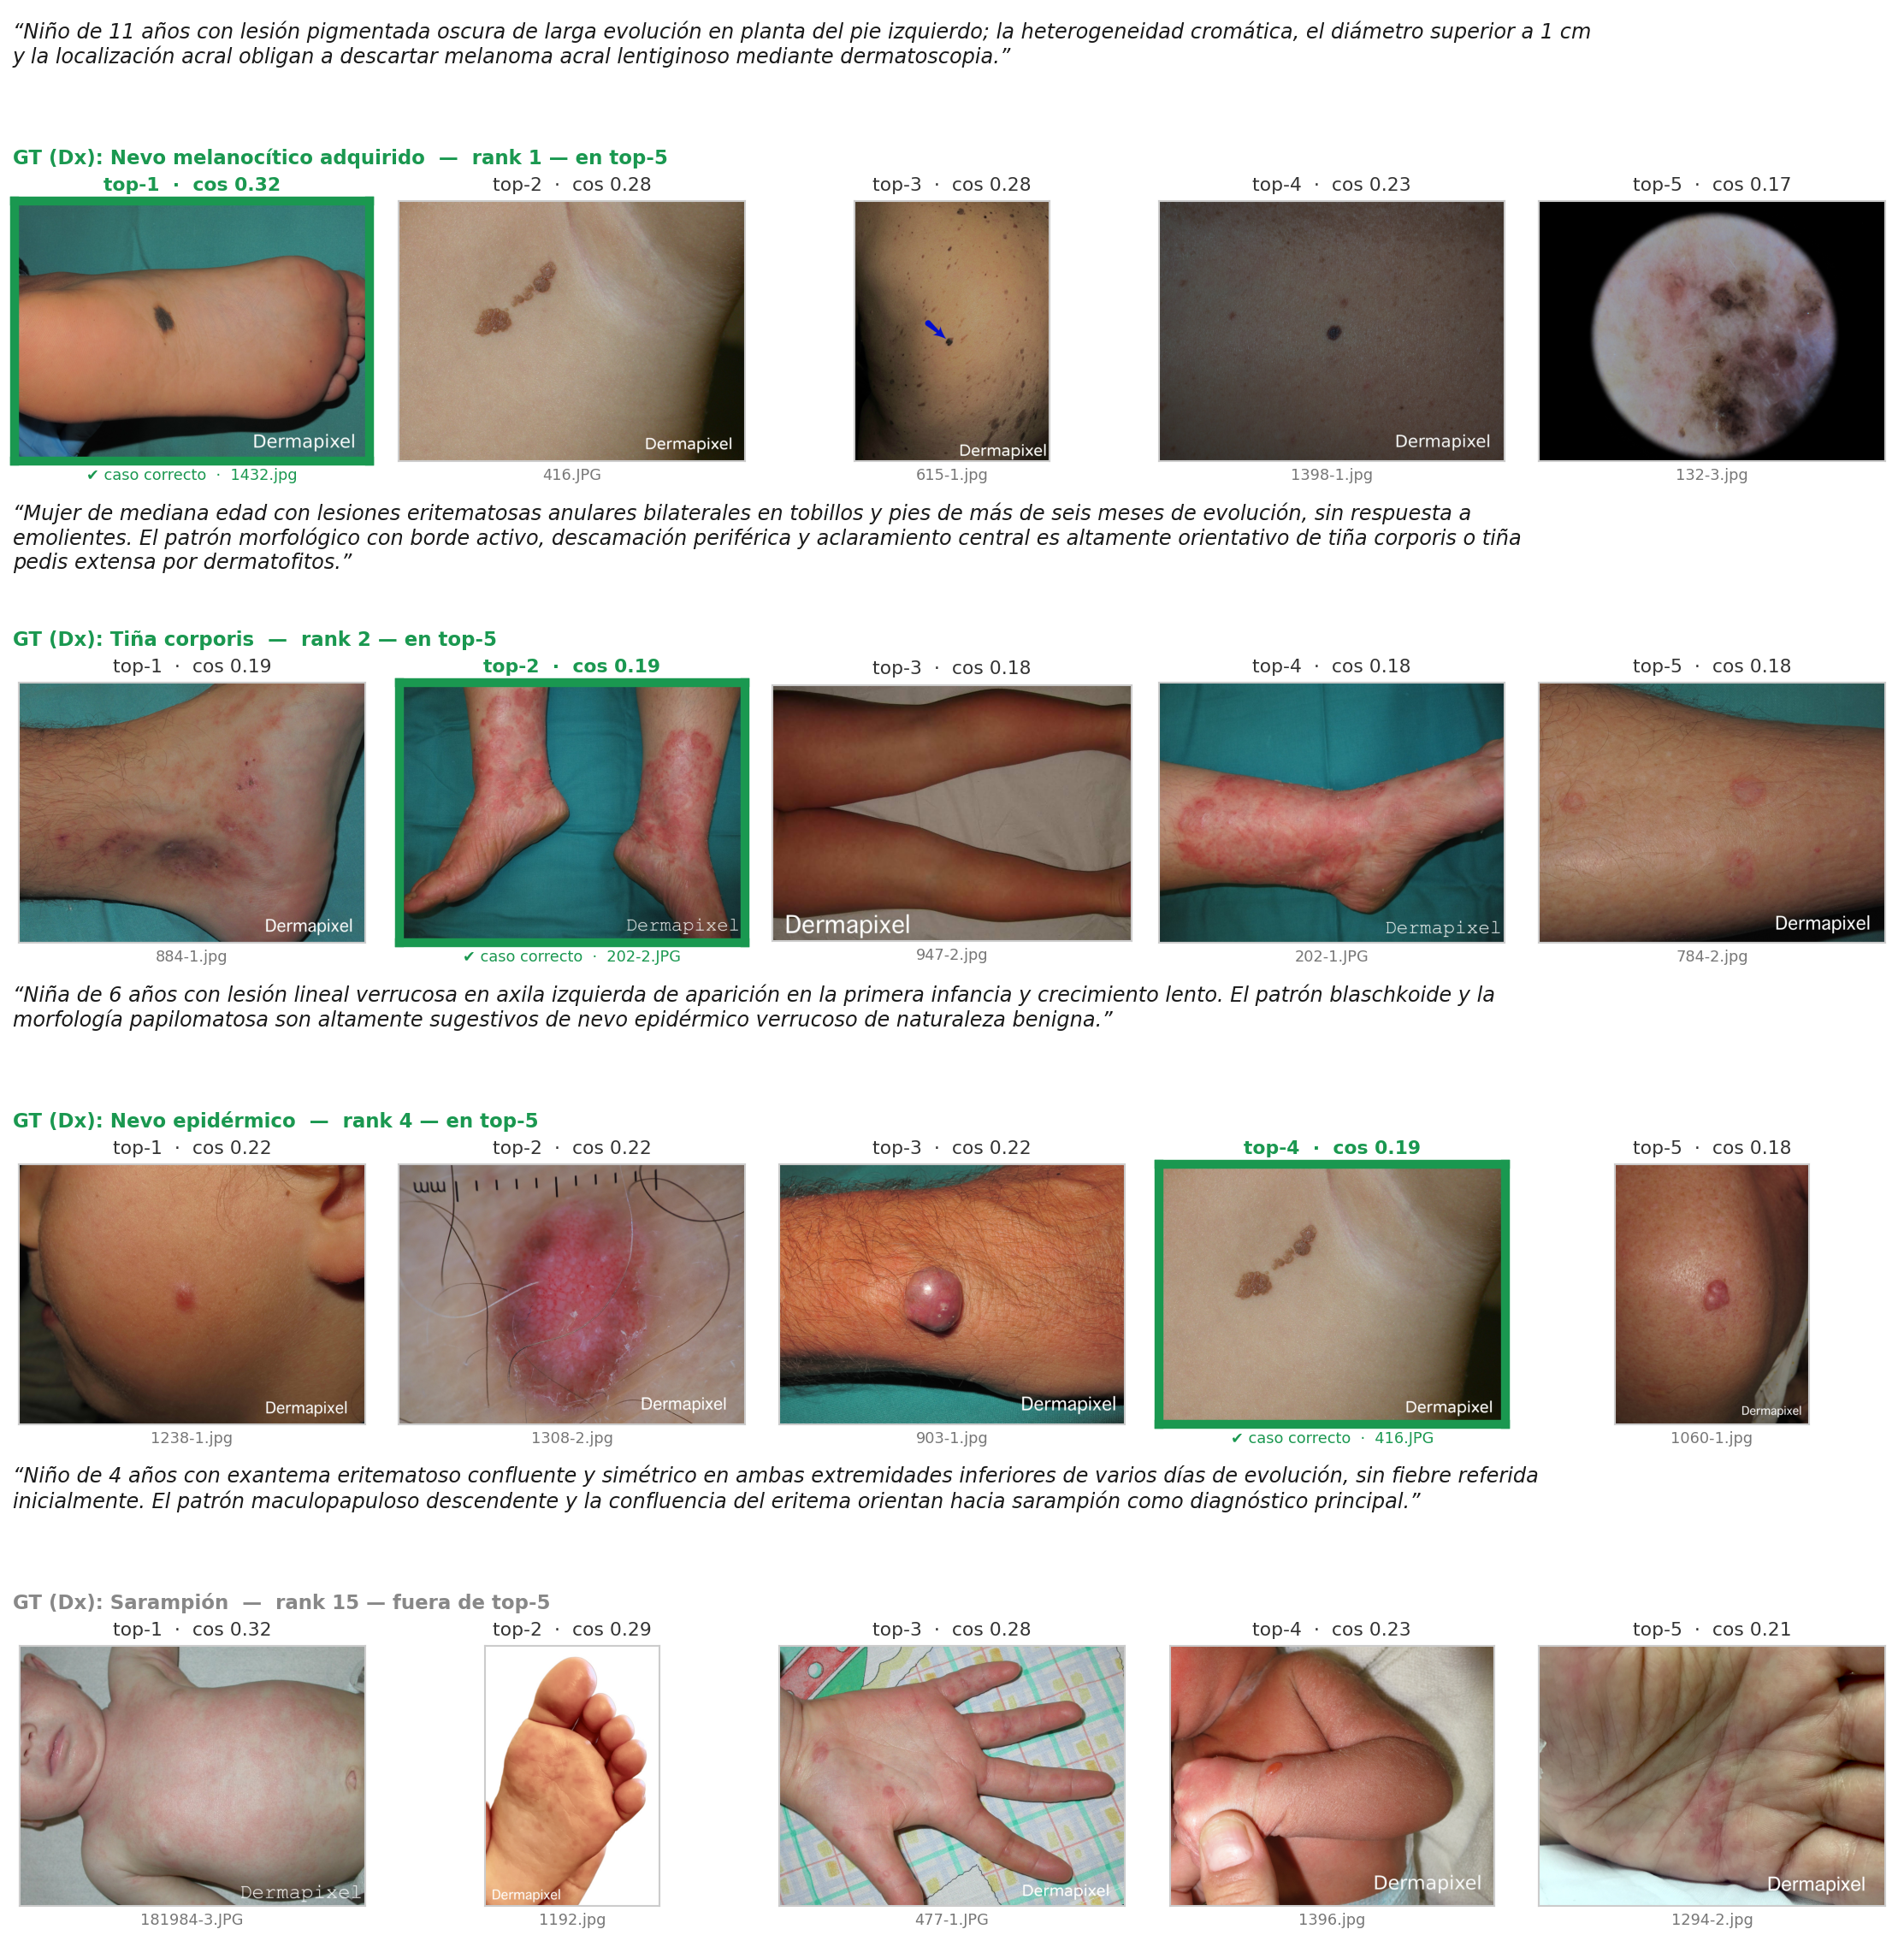
\includegraphics[width=\textwidth]{fig_retrieval_es.png}
\caption{Recuperación cross-modal texto$\to$imagen en castellano con la
rama contrastiva de Dermapixel R0 (checkpoint de mejor recuperación,
v2; régimen \emph{rich-caption} sobre los $107$ pares de validación).
Cada fila es una consulta de texto libre ---un resumen clínico real del
registro de la Dra.~R.~Taberner--- y sus cinco imágenes recuperadas por
similitud coseno; el marco verde señala el caso correcto (\emph{ground
truth}). Tres de las cuatro consultas recuperan el caso correcto en el
\emph{top-5}, en línea con la métrica global i2t R@$5 = 0{,}654$; la
última (exantema de sarampión) es un fallo honesto (rango $15$). Esta
métrica corresponde al régimen de validación con descripción rica y no
representa el uso real (consulta corta sobre el archivo completo), donde
la recuperación cae a niveles de azar.}
\label{fig:retrieval-es}
\end{figure}

\section{Síntesis comparativa de métodos sobre DermapixelAI 1.0}
\label{sec:dermapixel-extra}
\label{sec:dermapixel-extra-sintesis}

A lo largo de las
secciones~\ref{sec:dermapixel-results}--\ref{sec:spanderm-clip} se han
evaluado, sobre DermapixelAI~1.0, modelos especializados en dermatología
(PanDerm Base/Large, DermLIP v2), modelos médicos de imagen y texto
(BiomedCLIP, SigLIP-SO400M) y las dos ramas de Dermapixel R0. El
repositorio reproducible (\ref{cap:repo},
sección~\ref{sec:repo-ablaciones}) añade dos pruebas más, ya integradas
en esta síntesis: dos modelos generalistas no médicos (DINOv2, CLIP-L)
con linear probe y dos formas distintas de clasificar ---por vecinos más
cercanos (\emph{k}-NN con FAISS, es decir, asignar a cada imagen la clase
de los casos más parecidos del archivo) y zero-shot en cascada, decidiendo
primero la familia y luego el detalle---. La
tabla~\ref{tab:dermapixel-extra-sintesis} reúne BAcc y AUROC por nivel
para el conjunto completo de métodos.

\begin{table}[htbp]
\centering
\footnotesize
\setlength{\tabcolsep}{4pt}
\renewcommand{\arraystretch}{0.95}
\caption{Síntesis de encoders y arquitecturas evaluados sobre
DermapixelAI~1.0 (test fijo: $N = 36$ en L1/L2, $N = 28$ en L3).
La columna \emph{Ref.} remite a la sección de origen de las cifras
completas con sus intervalos de confianza. Mejor valor por columna
y nivel en negrita.}
\label{tab:dermapixel-extra-sintesis}
\begin{tabular}{llrrrrrr}
\hline
                                  &     & \multicolumn{2}{c}{L1} & \multicolumn{2}{c}{L2} & \multicolumn{2}{c}{L3} \\
Método                            & Ref.& BAcc & AUROC           & BAcc & AUROC           & BAcc & AUROC \\
\hline
PanDerm Base LP                   & \ref{sec:dermapixel-results} & $0{,}570$          & $0{,}697$
                                          & $0{,}221$          & $0{,}707$
                                          & $0{,}132$          & $0{,}735$ \\
PanDerm Large LP                  & \ref{sec:dermapixel-results} & $\mathbf{0{,}735}$ & $\mathbf{0{,}796}$
                                          & $0{,}265$          & $0{,}793$
                                          & $0{,}184$          & $0{,}813$ \\
DermLIP v2 LP                     & \ref{sec:dermapixel-results} & ---                & ---
                                          & ---                & $0{,}860$
                                          & ---                & --- \\
DINOv2 ViT-L LP                   & Rep.~\ref{sec:repo-ablaciones} & $0{,}537$          & $0{,}650$
                                          & $0{,}250$          & $0{,}718$
                                          & $0{,}211$          & $0{,}794$ \\
CLIP-L-336 LP                     & Rep.~\ref{sec:repo-ablaciones} & $0{,}556$          & $0{,}658$
                                          & $0{,}279$          & $\mathbf{0{,}826}$
                                          & $0{,}184$          & $\mathbf{0{,}827}$ \\
Dermapixel R0 LoRA                & \ref{sec:dermapixel-spanderm-v0} & ---                & ---
                                          & $\mathbf{0{,}363}$ & $0{,}855$
                                          & ---                & --- \\
FT parcial denso L1$+$L2$+$L3      & \ref{sec:dermapixel-results} & $0{,}622$          & $0{,}715$
                                          & $0{,}324$          & $0{,}852$
                                          & $0{,}184$          & $0{,}804$ \\
$k$-NN FAISS PanDerm Large         & Rep.~\ref{sec:repo-ablaciones} & $0{,}686$          & $0{,}748$
                                          & $0{,}265$          & $0{,}700$
                                          & $\mathbf{0{,}210}$ & $0{,}719$ \\
\hline
\end{tabular}
\end{table}

Ningún método gana en todo sobre DermapixelAI~1.0: quién va primero
cambia con el nivel de detalle (L1--L3) y con la métrica que se mire
---acierto equilibrado entre clases (BAcc), capacidad de ordenar bien los
casos (AUROC) o calidad de la búsqueda por parecido---, como refleja el
baile de negritas en la tabla~\ref{tab:dermapixel-extra-sintesis}. Como
las cifras salen del test fijo ($N = 36$ en L1/L2, $N = 28$ en L3), las
clasificaciones en L2 y L3 conviene tomarlas como indicio y contrastarlas
con la validación cruzada agrupada por caso
(tabla~\ref{tab:dermapixel-cv}), que es la estimación más fiable. En
resumen, cuál es la mejor opción depende del nivel que se quiera predecir
y de para qué se vaya a usar el sistema ---clasificar, buscar casos
parecidos o dar una explicación---, en la línea de la lectura
interpretativa de la sección~\ref{sec:disc-especializacion}.

Por último, con un enfoque orientado a la seguridad clínica, se probó a
\emph{combinar} un modelo dermatológico con uno generalista para no pasar
por alto ningún melanoma (maximizar la sensibilidad). Como es una
característica del prototipo y no un resultado central sobre modelos
fundacionales, los detalles ---configuración, tabla comparativa y
análisis de en qué se complementan--- están en el repositorio
reproducible (\ref{cap:repo}, sección~\ref{sec:repo-prototipo}).
